
\chapter{Introduction}
\label{chap:Intro}
\section{Polymorphism}
Polymorphism is the ability of a molecular solid, composed of the same molecular moieties, to exist in two or more crystalline conformations. These crystal conformations are called polymorphs and will transition from one to another under specific conditions, \autoref{polymorph_fig}. When polymorphism was first reported in 1832 by Friedrich Wçhler and Justus von Liebig, it was believed to affect only large, flexible molecules, such as proteins. However, as studies continued, it was discovered that over 50\% of molecules experience polymorphism \citep{cruz-cabeza_facts_2015,Hoja}.

\begin{figure}[ht]
    \centering
    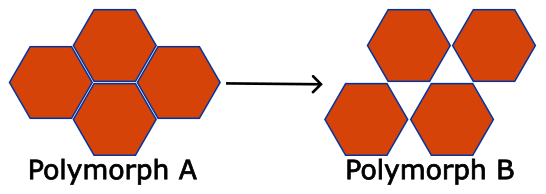
\includegraphics[width=12cm]{src/figures/intro_figs/polymorphism_fig.png}
    \caption{Diagram of a polymorphic phase transition from Polymorph A to Polymorph B.}
    \label{polymorph_fig}
\end{figure}

Due to the abundance of polymorphs and the influence of their crystalline structure on the intermolecular interactions present in a material, polymorphs and solvatomorph have become a widely growing area of study in fields of pharmaceutical development, crystal engineering, and de-novo materials design. Solvatomorphs are a specific class of polymorphs in which the solvent molecules crystallize with the solute molecules, see \autoref{solvatomorph_fig}. The system's intermolecular interactions are responsible for many of the substance’s properties, and can cause differences in solubility, vibrational spectra, densities, dissolution rate, melting point, mechanical properties, etc between crystal motifs \citep{Brittain2016,bernstein_polymorphism_2011,gentili_polymorphism_2019, Hoja}. Particularly difficult to characterize, hydrates are also a commonly observed branch of crystalline materials. Hydrates are a class of solvatomorphs in which at least one water molecule crystallizes within the unit cell with the solute molecules. These water molecules make studying polymorphism particularly difficult because of the extra degree(s) of freedom the molecules have when crystallizing and transitioning between polymorphs. In this study, we discuss our investigation of the possible polymorphism of barbituric acid dihydrate (BTADH) and violuric acid monohydrate (VAMH) using density functional theory (DFT). 
\begin{figure}[ht]
    \centering
    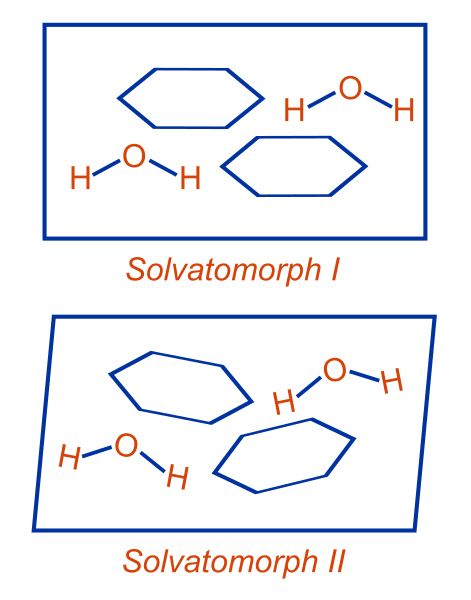
\includegraphics[width=8cm]{src/figures/intro_figs/solvatomorphs.png}
    \caption{Diagram of Solvatomorphs.}
    \label{solvatomorph_fig}
\end{figure}
\section{Density Functional Theory}
Density functional theory is a method of analysis that utilizes first principle, quantum mechanics calculations to investigate the electronic structure of materials \citep{baseden_introduction_2014,paul_true_2019}. Many physical and chemical properties are governed by the material's electronic states. DFT calculations provide accurate information about your system because the calculations take into account quantum mechanical effects, however, this trade-off in accuracy comes at a high computational cost compared to other simulation methods. DFT uses the electron density surrounding a particle to calculate the energy. The particles undergo a slight change in position and the energies are calculated again. This continues until the system's energy is at a minimum. 

\begin{figure}
    \centering
    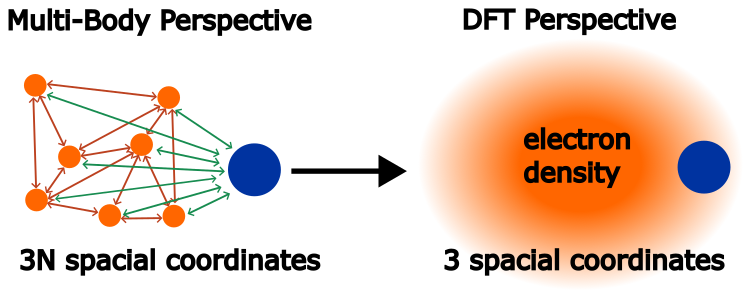
\includegraphics[width=12cm]{src/figures/intro_figs/dft_diagram.png}
    \caption{A depiction of how density functional theory simplifies the many-body problem into a function of electron density. }
    \label{DFT_diagram}
\end{figure}

DFT was developed upon the Hohenberg-Kohn theorems, the first of which was published in 1964 \citep{hohenberg_inhomogeneous_1964}. The first theorem states that the ground state properties, or energies, of a many body system can be calculated using only a functional ($F[n]$) of the electron density ($n(\textbf{r})$). This theorem reduced the many body problem of N particles from 3N spacial coordinates down to only 3 spacial coordinates. The electron density is defined in terms of the three spacial coordinates, shown in \autoref{DFT_diagram}. While the first theorem describes the possibility of calculating ground state properties from electron density it does not provide any information about the functional required to do so. The second Hohenberg-Kohn theorem states that if the exact functional of a system is known, the electron density that minimizes this functional will correspond to the exact solution of the Scrhodinger's equation \citep{kohn_self-consistent_1965}. Though the only system in which an exact functional has been proven is for a homogeneous electron gas, in all many-body systems the energy functional must be approximated. 
\subsection{Functionals and Basis Sets}
\autoref{eq_dft1} describes DFT in a mathematical sense, where $E_{v}[n]$ is equal to the ground state energy of the system and $v(\textbf{r})$ is the external potential. \autoref{eq_dft1} also details that the density functional $F[n(\textbf{r})]$ is independent of the external potential. 
\begin{equation}
    E_{v}[n] \equiv \int v(\textbf{r}) n(\textbf{r})d\textbf{r} + F[n(\textbf{r})]
    \label{eq_dft1}
\end{equation}
We can further examine the total energy of the system using \autoref{eq_dft2}. 
\begin{equation}
    E[\{\Psi_i\}] \equiv E_{known} [\{ \Psi_i \}] + E_{XC} [\{\Psi_i\}]
    \label{eq_dft2}
\end{equation}
The $E_{known}$ term includes the kinetic, potential, and hartree energy, all of which can be calculated exactly for a given system. The second term of \autoref{eq_dft2} includes the exchange-correlation energy $E_{XC}$. This energy is unknown for many-body systems and therefore has to be approximated using density functionals. The exchange-correlation energy can only be calculated for a homogeneous, uniform electron gas, with constant electron density, which is the system that Hohenberg and Kohn used to prove their first theorem, mentioned above \citep{hohenberg_inhomogeneous_1964}. Different systems may require different approximations, depending on the information you are trying to learn from your simulation. This makes choosing your functional one of the most important steps in a DFT investigation. For more complex systems various types of functionals exist, including the local density approximation (LDA), generalized gradient approximation (GGA) and hybrid functionals, among others \citep{goh_exchange-correlation_nodate, hasnip_density_2014}. LDA functionals are the most simplified models, they take into account only the electron density derived from a free electron gas. GGA functionals build on LDA functionals by also including information about the gradient observed in the electron density. This adds a level of complexity and accuracy for models that do not have uniform electron density. The functionals used in this body of work are hybrid functionals. Hybrid functionals combine the exact electron density of the system, derived by the Hartree-Fock theory, with the $E_{XC}$ from traditional DFT functionals, such as the GGA \citep{hybrid_2007, Heda_2023}. 
Along with choosing the functional, you must also determine a basis set to use in your DFT calculations. The basis set is set of basis functions that reduces calculations from partial derivatives to algebraic equations. Various types of basis sets exist, including plane-wave and atomic orbital. Atomic orbital basis sets place the basis equations on each atom in order to build the atomic orbitals. 
Chapters 2 and 3 detail how DFT was utilized to determine the crystalline configurations of two hydrate systems, violuric acid monohydrate and barbituric acid dihydrate, over a broad temperature range. Both hydrate systems had been suspected to exhibit polymorphism, but upon further investigation it was concluded that crystalline disorder was skewing the experimental results and the accurate crystalline configurations were determined using DFT geometry optimization calculations. 

\section{Organic Photovoltaics}
Photovoltaic (PV) devices are a promising solution to the rising energy crisis in America \citep{mazzio_future_2015}. Inorganic photovoltaic cells, often composed of silicon, have a relatively high production and implementation cost\citep{mazzio_future_2015}. Producing organic photovoltaic devices (OPVs) can be done at a potentially lower cost than silicon because the raw materials require less energy-intensive processing. Small molecule OPVs have recently achieved a photoelectric efficiency of almost 20\%, which has increased impressively over recent years \citep{sun_span_2022}. The Shockley-Quiesser limit suggests that there is still room for the power conversion efficiency of organic solar devices to increase by approximately 15\%, leading to a PCE of 35\% \citep{miller_strong_2012}. Introducing morphologies that have a higher charge carrier mobility have been proven to be the key to improving the cell’s PCE. 
Organic materials are typically not thought of as semiconductors, however, it is evident throughout biology that many organic molecules can function as semiconductors. For an organic material to act as a semiconductor the molecules must exhibit significant conjugation \citep{kularatne_donoracceptor_2013}. Conjugation is the presence of overlapping pi-orbitals that create a system of delocalized electrons. These delocalized electrons are more readily excitable and are not linked to one specific atom within the molecule. As the conjugation length increases in the material, the band gap decreases, meaning that the electrons require less energy to be excited into the conduction band. Once in the conduction band the electron can contribute to conductivity \citep{callister_materials_2010}. In order to excite an electron from the highest occupied molecular orbital (HOMO) to the lowest unoccupied molecular orbital (LUMO) the incident photon’s energy must be equal to or greater than the excitation energy. When an electron is excited into the LUMO, where it has enough energy to move about the surface of the molecule, there is a leftover ‘hole’ where the electron used to be. In comparison the the negative environment surrounding it, the hole has an effective positive partial charge. The electron and hole have a coulombic attraction due from their opposing charges, resulting in a force that binds the electron and hole together into what is called an exciton \citep{reis_effect_2022}.
\begin{figure}[ht]
    \centering
    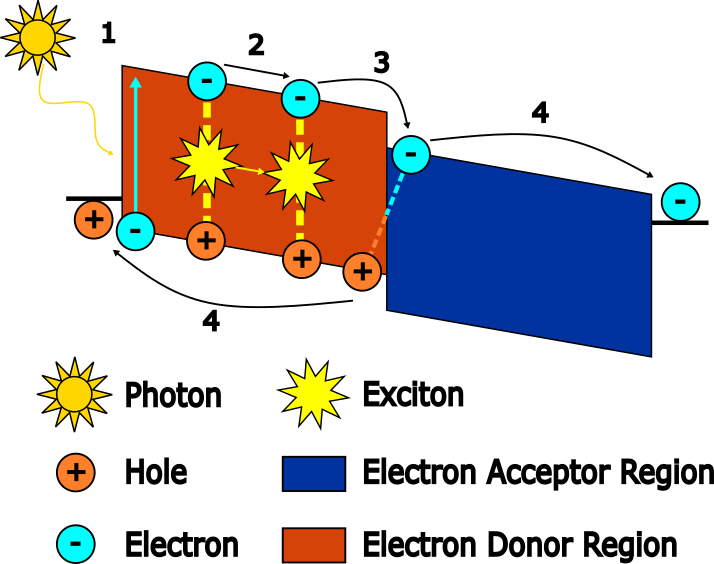
\includegraphics[width=10cm]{src/figures/intro_figs/OPV_Figure.png}
    \caption{Diagram of an OPV device. (1) Photon absorption (2) Exciton creation and migration (3) Exciton dissociation (4) Charge carrier diffusion.}
    \label{OPV_fig}
\end{figure}
\par The photoelectric effect, described above, is what makes OPV devices functional. In an OPV device, when an incident photon hits the surface it is passed through into the active layer, where an exciton is created (\autoref{OPV_fig}, step 1). The exciton diffuses through the active layer until it reaches a grain boundary between an acceptor region and donor region, where exciton dissociation occurs (\autoref{OPV_fig}, steps 2 \& 3). Once the coulombic connection between the electron and hole is broken the electron diffuses through the acceptor region to be harvested at the cathode and the hole through the donor region to be harvested at the anode (\autoref{OPV_fig}, step 4) \citep{Zhang2018}. 
\begin{wrapfigure}{r}{0.5\textwidth}
  \begin{center}
    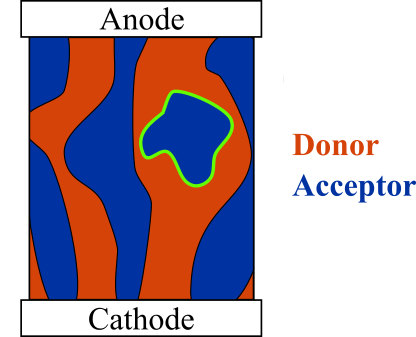
\includegraphics[width=0.48\textwidth]{src/figures/intro_figs/bulk_heterojunction.png}
  \end{center}
    \caption{Depiction of a bulk heterojunction (BHJ) active layer of an organic photovoltaic device. Outlined in green is a an "island" where the electron would have no access to the electrode, forcing it to recombine with a hole, rendering it useless.}
  \label{BHJ}
\end{wrapfigure}
\par The active layer motif depicted in \autoref{BHJ} is called a bulk heterojunction active layer \citep{gaspar_recent_2018}. These donor/acceptor regions can come from two different organic semiconductor molecules or a co-polymer with differing acceptor monomers and donor monomers \citep{piris_photogeneration_2009}. The donor/acceptor regions need to exhibit a significant difference in energy levels in order to cause exciton dissociation when the exciton crosses the grain boundary. Once the excitons are dissociated the charge carriers have to pass through the active layer to their respective anodes \citep{radford_controlling_2021}. If there is not a clear path for the electron or hole to travel to electrodes these charges are typically lost to exciton recombination. This is why the morphology of the active layer is so important to the power conversion efficiency. 
\par Understanding the influence of structural conformation on OPV device performance brings us to the importance of density functional theory calculations and molecular dynamics simulations. DFT has many applications, one of which is geometry optimizations of small molecule systems. From these geometry optimizations we can determine the most energetically favorable conformation of our system. Molecular dynamics (MD) simulations (as discussed below) are an efficient way to determine the morphology of the active layer and the properties associated with it \citep{chen_fluorination_2022}. MD simulations are used for investigating the structures of OPV active layers because they follow the self-assembly of the copolymers in a bulk heterojunction. MD simulations give us information about the thermodynamics of the self-assembly as well as the kinetics of how these molecules interact to form the equilibrium structures. MD simulations also have the benefit of simulating large molecule systems at a lower computational cost than DFT. The information gained from DFT calculations in conjunction with MD simulations can give great insight into how our copolymers will self-assemble during in the active layer during device production \citep{krebs_all_2009}. 

\section{Molecular Dynamics}
\par Molecular dynamics is a computational simulation method used to predict equilibrium morphologies of many particle systems. Newton's equations of motion are solved numerically to generate trajectories of how molecular systems evolve over time \citep{frenkel_understanding_2002}. 
The basic algorithm behind an MD simulation is: (1) calculate potentials and forces from particle positions. (2) Update particle velocities using the forces calculated in (1). (3) Update particle positions from the velocities calculated in (2). (4) Continue (1)-(3) with updated particle positions until equilibrium is achieved. 
Once equilibrium is achieved we  calculate the decorrelation time (time steps between independent samples) and calculate system properties by averaging independent microstates. 
\par The forces of attraction and repulsion enacted on one particle by another are described by the particles' pair potential. The pair potential is essentially the potential energy of two interacting particles. A common pair potential used in MD simulations is the Lennard-Jones (LJ) potential \citep{vollmayr-lee_introduction_2020,LJ_history}. The LJ-potential, depicted in \autoref{ljplot} and explained mathematically in \autoref{lj-equation}, describes the potential energy $U_{LJ}(r_{i,j})$ of two particles, $i$ and $j$, as a function of internuclear distance, $r_{i,j}$. 
\begin{figure}[ht]
    \centering
    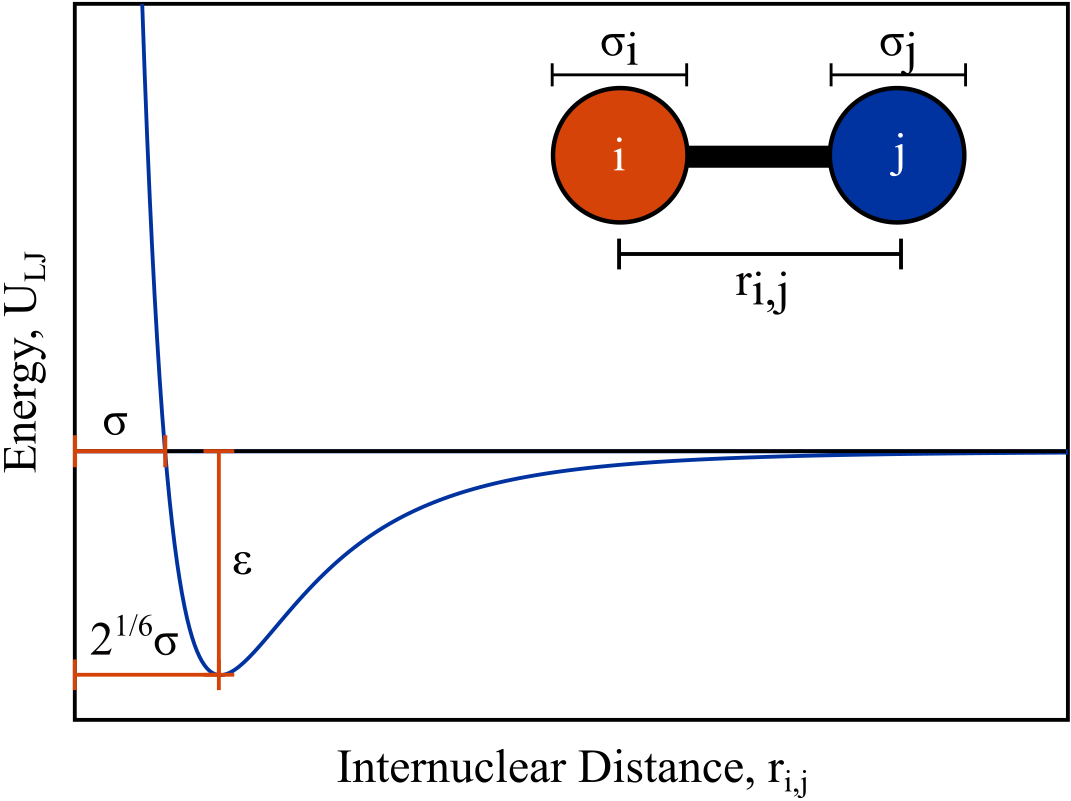
\includegraphics[width=12cm]{src/figures/intro_figs/LJ_pot.png}
    \caption{Plot of the Lennard-Jones potential energy.}
    \label{ljplot}
\end{figure}

\begin{equation}
    U_{LJ}(r_{ij}) = 4\epsilon \left[ \left({\frac{\sigma}{r_{ij}}}\right)^{12} - \left({\frac{\sigma}{r_{ij}}}\right)^{6} \right]
    \label{lj-equation}
\end{equation}

Pair interactions are governed by $\sigma$ and $\epsilon$. $\sigma$ is the internuclear distance at which the potential energy between two particles is zero and epsilon is the depth of the well in the potential energy plot. $\epsilon$ is a measure of how attractive the particle is and $\sigma$ can be thought of as the diameter of the particle. As shown in \autoref{ljplot}, the potential energy reaches a minimum when the particles are at a distance of $2^{1/6}\sigma$ apart. At distances closer than $2^{1/6}\sigma$, the particles repel one another and at distances greater than $2^{1/6}\sigma$ the the forces felt are negative, which accelerates the particles toward one another. The greater the distance gets from $2^{1/6}\sigma$, the lesser the effect the attractive force has on the other particle. In this study, we used the Lorentzian combination rule for sigma and a geometric combining rule for epsilon, shown in \autoref{comb_rule}. 

\begin{equation}
    \sigma_{i,j} = \frac{\sigma_{i} + \sigma{j}}{2}  ,   \epsilon_{i,j} = \sqrt{\epsilon_{i} * \epsilon_{j}}
    \label{comb_rule}
\end{equation}

Other properties, such as bond, angle and dihedral, also dictate how particles interact and how a system evolves over time. In MD simulations bonds and bond angles are described as harmonic oscillators, using \autoref{potE_bond_distance}, where $U(r)$ is the potential energy of the bond, $r$ is the internuclear distance between the bonded particles, $r_0$ is the equilibrium internuclear distance and $k_h$ is the bond's harmonic spring constant. A diagram depicting the bonds, angles, and dihedral angles is shown in \autoref{forces_fig}. 

\begin{equation}
    U(r) = \frac{1}{2} k_{h} \left( r - r_{0} \right)
    \label{potE_bond_distance}
\end{equation}
\autoref{potE_bond_angle} described the potential energy $U(\theta)$ associated with the bond angle, $\theta$, where $\theta_0$ is the equilibrium bond angle and $k_{\theta}$ is the harmonic angle constant. 
\begin{equation}
    U(\theta) = \frac{1}{2} k_{\theta} (\theta - \theta_{0})
    \label{potE_bond_angle}
\end{equation}
\begin{figure}[ht]
    \centering
    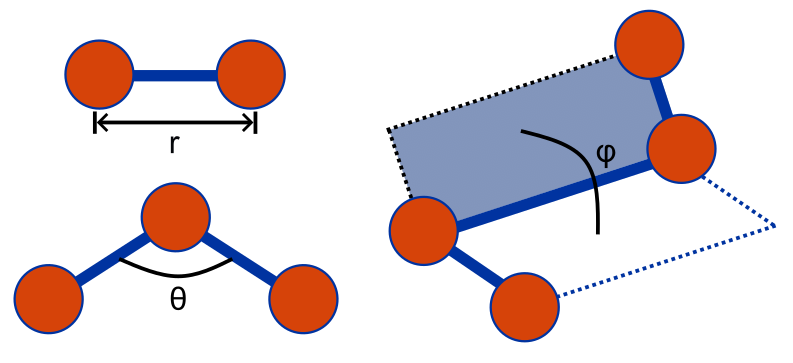
\includegraphics[width=0.5\linewidth]{src/figures/intro_figs/dihedral_fig.png}
    \caption{Illustration of bond distance (r), bond angle ($\theta$), and dihedral angle ($\phi$)}.
    \label{forces_fig}
\end{figure}
\par Dihedrals are described using \autoref{potE_dihedral}, where $k_n$ is the spring constant of the corresponding particle, $\phi$ is the angle between atoms planes within the dihedral, and $U(\phi)$ is the potential energy of the dihedral. 

\begin{equation}
    U(\phi) = \frac{1}{2}k_1(1+\cos(\phi)) + \frac{1}{2}k_2(1+\cos(2\phi)) + \frac{1}{2}k_3(1+\cos(3\phi)) + \frac{1}{2}k_4(1+\cos(4\phi))
    \label{potE_dihedral}
\end{equation}

In our simulation framework we try to follow the TRUE model, ensuring that our simulations are transparent, reproducible, usable and extensible. In MD simulations a forcefield is used to efficiently store and keep track of all the variables used in the pair, angle, bond, harmonic potentials mentioned above \citep{ghahremanpour_refinement_2022,gaff}. Each unique pair interaction requires its own unique set of parameters to model the pair of particles using the equations listed above. The process of creating and applying a forcefield is a common barrier to the transparency and reproducibility of our TRUE simulations \citep{jankowski_perspective_2020}. It is frequent in initializing a simulation of a new molecule to have missing forcefield parameters. In these cases the parameters must be either added to an existing forcefield file or a new forcefield file must be produced. In this study, we have developed a workflow that implements an open source software to create a forcefield file from a molecule graph \citep{wang_end--end_2022}. We have validated this workflow for complex, conjugated polymers by comparing simulation results of two molecules to previously published results (Chapter 4). After validating this workflow it was utilized to simulate 13 different complex polymers (Chapter 5).  

In comparison to MD simulations, DFT calculations come with a much higher computational cost. Due
to this, larger systems that can be equilibrated using MD cannot be simulated with DFT. On the other
hand, however, MD simulations often don’t provide as much information about a system as DFT
calculations do. This is due to the neglect of quantum effects in MD simulations. Due to these differences, in this dissertation we utilize DFT to predict the crystalline conformation of small molecules like BTADH and VAMH, but employ MD simulations to determine how macromolecules and polymers interact to self-assemble into bulk morphologies. In both cases, however, molecular simulations are used over experiment due to experimental constraints, such as difficulty in structure determination and experimental costs and time. The results from the molecular simulations are then used to direct experimental research toward materials of interest for the given application. 